\documentclass[11pt]{article}

\usepackage[utf8]{inputenc}
\usepackage[T1]{fontenc}
\usepackage[ngerman]{babel}
\usepackage[a4paper,margin=0.85in]{geometry}
\usepackage{graphicx}
\usepackage{array}
\usepackage{parskip}
\usepackage{ragged2e}

\pagestyle{empty}
\renewcommand{\baselinestretch}{1.0}

\begin{document}

% ---------- Title ----------
\begin{center}
    {\Large \textbf{Bewerbung}} \\[3cm]
    
    {\Huge \textbf{Zhongli Wang}} \\[0.4cm]
    
    {\huge Bewerbung als Data Scientist} \\[0.25cm]
    {\large Quantitative Medienforschung, R, Statistik \& KI}
\end{center}

\vspace{0.6cm}

% ---------- Large Picture in the Middle ----------
\begin{center}
    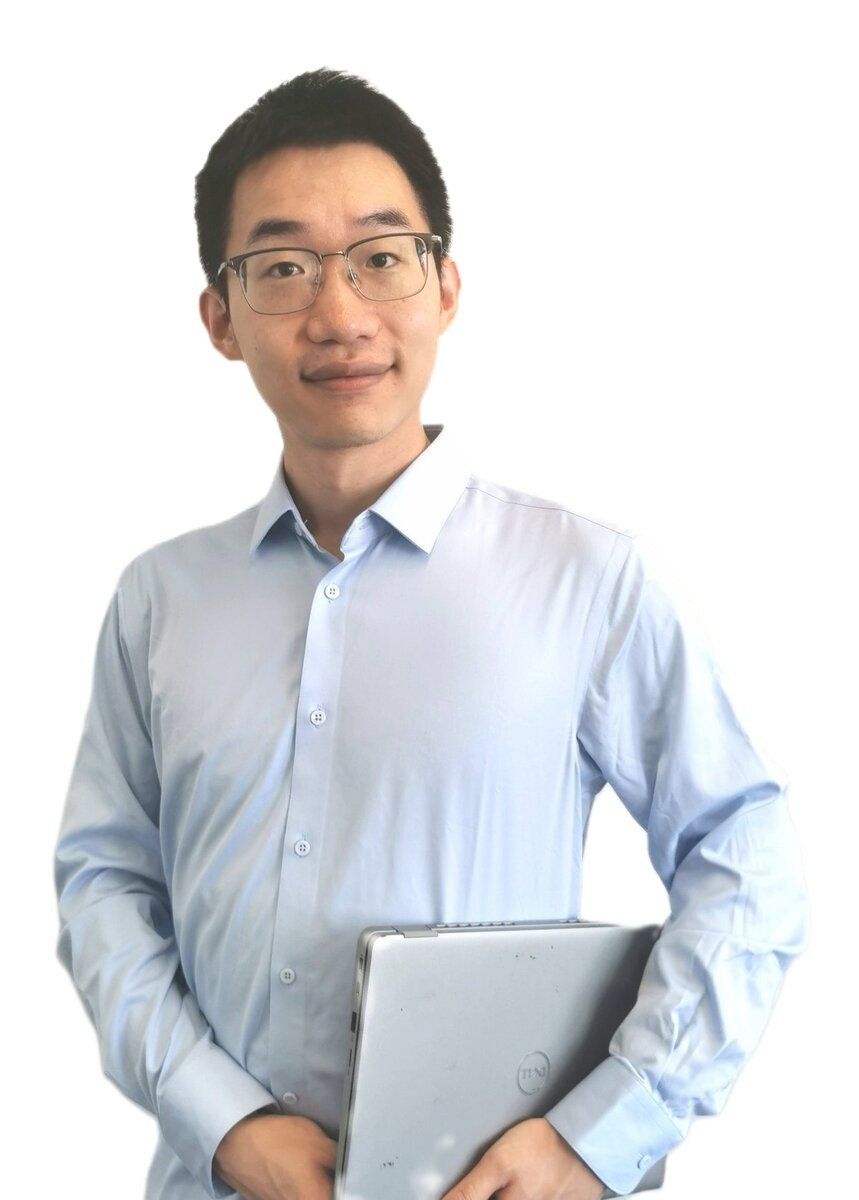
\includegraphics[
        width=0.55\textwidth,
        height=0.45\textheight,
        keepaspectratio
    ]{../../zhongli-wang-profile.jpg}
\end{center}

\vspace{0.7cm}

% ---------- Personal Details ----------
\begin{center}
\renewcommand{\arraystretch}{1.35}
\begin{tabular}{>{\bfseries}p{4.2cm} p{8.5cm}}

Anschrift: & Astastrasse 22, 33617 Bielefeld, Deutschland \\

Telefon: & +49 160 9541 6015 \\

E-Mail: & nkwangzhongli@gmail.com \\

\end{tabular}
\end{center}

\vfill

\newpage

\begin{flushright}
Zhongli Wang \\
Astastrasse 22 \\
33617 Bielefeld \\
Deutschland \\
\end{flushright}

\vspace{0.1cm}

\noindent
Recruiting-Team \\
ANKORDATA GmbH \& Co. KG \\
Frankfurt am Main \\

\vspace{0.05cm}

\noindent
\textbf{Bewerbung als Data Scientist: Quantitative Medienforschung, R, Statistik \& KI}

\noindent Sehr geehrtes Recruiting-Team,

bei ANKORDATA möchte ich meine Erfahrung in statistischer Modellierung und maschinellem Lernen für verlässliche Analysen in der quantitativen Medienforschung einsetzen. 
An Ihrem Methodenansatz interessiert mich besonders, wie Gewichtung, Imputation und Reichweitenmodellierung zu automatisierten Verarbeitungsschritten verbunden werden. 
Ich suche eine Aufgabe, in der ich Methoden entwickeln, ihre Qualität prüfen und gemeinsam mit der Softwareentwicklung in laufende Datenprozesse überführen kann.

In meiner wirtschaftswissenschaftlichen Promotion an der Universität Bielefeld entwickle und untersuche ich agentenbasierte Modelle zu Unternehmensentscheidungen, 
Netzwerkeffekten und heterogenen Konsumenten. 
In einem Forschungsprojekt zur Parameterschätzung vergleiche ich die simulierte Momentenmethode mit neuronalen Surrogatmodellen. 
Meine Mitautorenschaft an \emph{Polytope Fraud Theory}, 
erschienen 2025 im \emph{International Review of Financial Analysis}, 
verbindet Finanzdatenanalyse mit überwachtem Lernen sowie Random Forest, Neural Networks, XGBoost, usw. zur Betrugserkennung. 
Diese Erfahrungen bilden meine Grundlage für die Prüfung von Modellannahmen und die Bewertung analytischer Ergebnisse.

Python nutze ich für Simulationen, Datenanalyse und Machine Learning mit scikit-learn; 
R gehört ebenfalls zu meinen Analysewerkzeugen. 
Bei ANKORDATA möchte ich reproduzierbare Analyseprozesse in R weiterentwickeln und mich gezielt in tidyverse und targets einarbeiten. 
Datenaufbereitung, Plausibilitätsprüfungen, nachvollziehbare Dokumentation und die sorgfältige Pflege bestehender Abläufe gehören für mich zu dieser Aufgabe.

Für KI-gestützte Forschungs- und Entwicklungsaufgaben arbeite ich mit Claude Code und LLM-Werkzeugen. Als Mitautor von \emph{Agentic Workflows for Economic Research} habe ich an einem Forschungsframework auf Basis von Microsoft AutoGen mitgewirkt. 
Diese Erfahrung möchte ich für effizientere Entwicklung und Dokumentation einbringen. 
Die spezifischen Verfahren der Medienforschung, insbesondere Gewichtung, Hochrechnung und Reichweitenmessung, möchte ich mir systematisch erschließen. 
Dabei bringe ich Deutsch- und Englischkenntnisse auf C1-Niveau sowie Erfahrung in der Vermittlung quantitativer Forschungsergebnisse mit.

Ich freue mich darauf, mit Ihnen zu besprechen, wie ich Ihre Methodenentwicklung und die Qualität Ihrer Datenprozesse unterstützen kann. Auch für einen Einstieg im Rahmen eines Praktikums bin ich offen.


\vspace{0.15cm}

\noindent Mit freundlichen Grü\ss{}en, \\
\vspace{2mm}\\
\noindent Zhongli Wang

\vspace{0.05cm}
\noindent
\includegraphics[width=2.7cm,keepaspectratio]{../../Wang-sig.jpg}

\end{document}
